\chapter{Formal Methodology and CertGraph Architecture}
\label{ch:methodology}

\section{Mathematical Formulation of Enterprise Identity Graphs}
To rigorously model the complex authorization topology of Active Directory and ADCS, we formalize the enterprise environment as a typed, directed, heterogeneous multigraph.

\begin{definition}[Active Directory Heterogeneous Multigraph]
An Active Directory environment is defined as a 6-tuple:
\begin{equation}
G = (V, E, \mathcal{T}_V, \mathcal{T}_E, \phi_V, \psi_E)
\end{equation}
where:
\begin{enumerate}
    \item $V = \bigcup_{\tau \in \mathcal{T}_V} V_\tau$ is the set of all directory entities (vertices).
    \item $E \subseteq V \times \mathcal{T}_E \times V$ is the multiset of directed authorization and administrative relationships (edges).
    \item $\mathcal{T}_V = \{\text{User}, \text{Computer}, \text{Group}, \text{Template}, \text{EnterpriseCA}\}$ represents the discrete set of node entity types.
    \item $\mathcal{T}_E = \{\text{MemberOf}, \text{Enroll}, \text{GenericAll}, \text{WriteDacl}, \text{WriteOwner}, \text{PublishedTo}, \text{ManageCA}, \text{LinksPolicy}\}$ represents the discrete set of relation types.
    \item $\phi_V: V \to \mathcal{T}_V$ is a type-mapping function assigning each vertex $v \in V$ its structural type $\tau(v)$.
    \item $\psi_E: E \to \mathcal{T}_E$ is a relation-mapping function assigning each edge $e = (u, r, v)$ its relation type $r$.
\end{enumerate}
\end{definition}

\subsection{Node Feature Vector Spaces}
Each vertex $v \in V$ is assigned an initial feature vector $x_v \in \mathbb{R}^{d_{\tau(v)}}$ encoding intrinsic local attributes extracted from LDAP:
\begin{enumerate}
    \item \textbf{Template Nodes ($x_{\text{Template}} \in \mathbb{R}^{10}$):} Feature vectors capture binary configuration flags:
    \begin{equation}
    x_{\text{Template}} = [f_{\text{supplies\_subject}}, f_{\text{client\_auth}}, f_{\text{any\_purpose}}, f_{\text{agent\_eku}}, f_{\text{no\_security\_ext}}, f_{\text{schema\_v1}}, f_{\text{requires\_approval}}, f_{\text{has\_policy\_link}}, f_{\text{has\_dangerous\_dacl}}, f_{\text{is\_published}}]^T
    \end{equation}
    \item \textbf{User and Computer Nodes ($x_{\text{User}} \in \mathbb{R}^6, x_{\text{Computer}} \in \mathbb{R}^6$):}
    \begin{equation}
    x_v = [f_{\text{is\_enabled}}, f_{\text{is\_sensitive}}, f_{\text{dont\_req\_preauth}}, f_{\text{trusted\_for\_delegation}}, f_{\text{has\_spn}}, f_{\text{is\_admin}}]^T
    \end{equation}
    \item \textbf{Group Nodes ($x_{\text{Group}} \in \mathbb{R}^2$):}
    \begin{equation}
    x_{\text{Group}} = [f_{\text{is\_high\_value\_tier0}}, f_{\text{is\_builtin}}]^T
    \end{equation}
    \item \textbf{Enterprise CA Nodes ($x_{\text{CA}} \in \mathbb{R}^3$):}
    \begin{equation}
    x_{\text{CA}} = [f_{\text{is\_root\_ca}}, f_{\text{allows\_user\_spec}}, f_{\text{enforces\_encryption}}]^T
    \end{equation}
\end{enumerate}

\subsection{Relational Adjacency and Canonical Relations}
For each relation type $r = (\tau_s, \text{rel}, \tau_t) \in \mathcal{T}_E$, the directed adjacency matrix $A_r \in \{0, 1\}^{|V_{\tau_s}| \times |V_{\tau_t}|}$ satisfies:
\begin{equation}
A_r[u, v] = 1 \iff (u, r, v) \in E
\end{equation}
Because information flow in GNNs must model both vulnerability propagation (from users to templates) and reverse privilege lookup (from templates to authorized users), we introduce reverse canonical relations $r^{-1} = (\tau_t, \text{rel}^{-1}, \tau_s)$ with transposed adjacency $A_{r^{-1}} = A_r^T$.

\section{The CertGraph Hetero-GAT Architecture}
CertGraph implements an inductive Heterogeneous Graph Attention Network (Hetero-GAT). Unlike homogeneous GNNs that collapse node and edge distinctions, CertGraph processes distinct linear transformations and attention projections for each canonical relation $r \in \mathcal{T}_E$.

\begin{figure}[t]
    \centering
    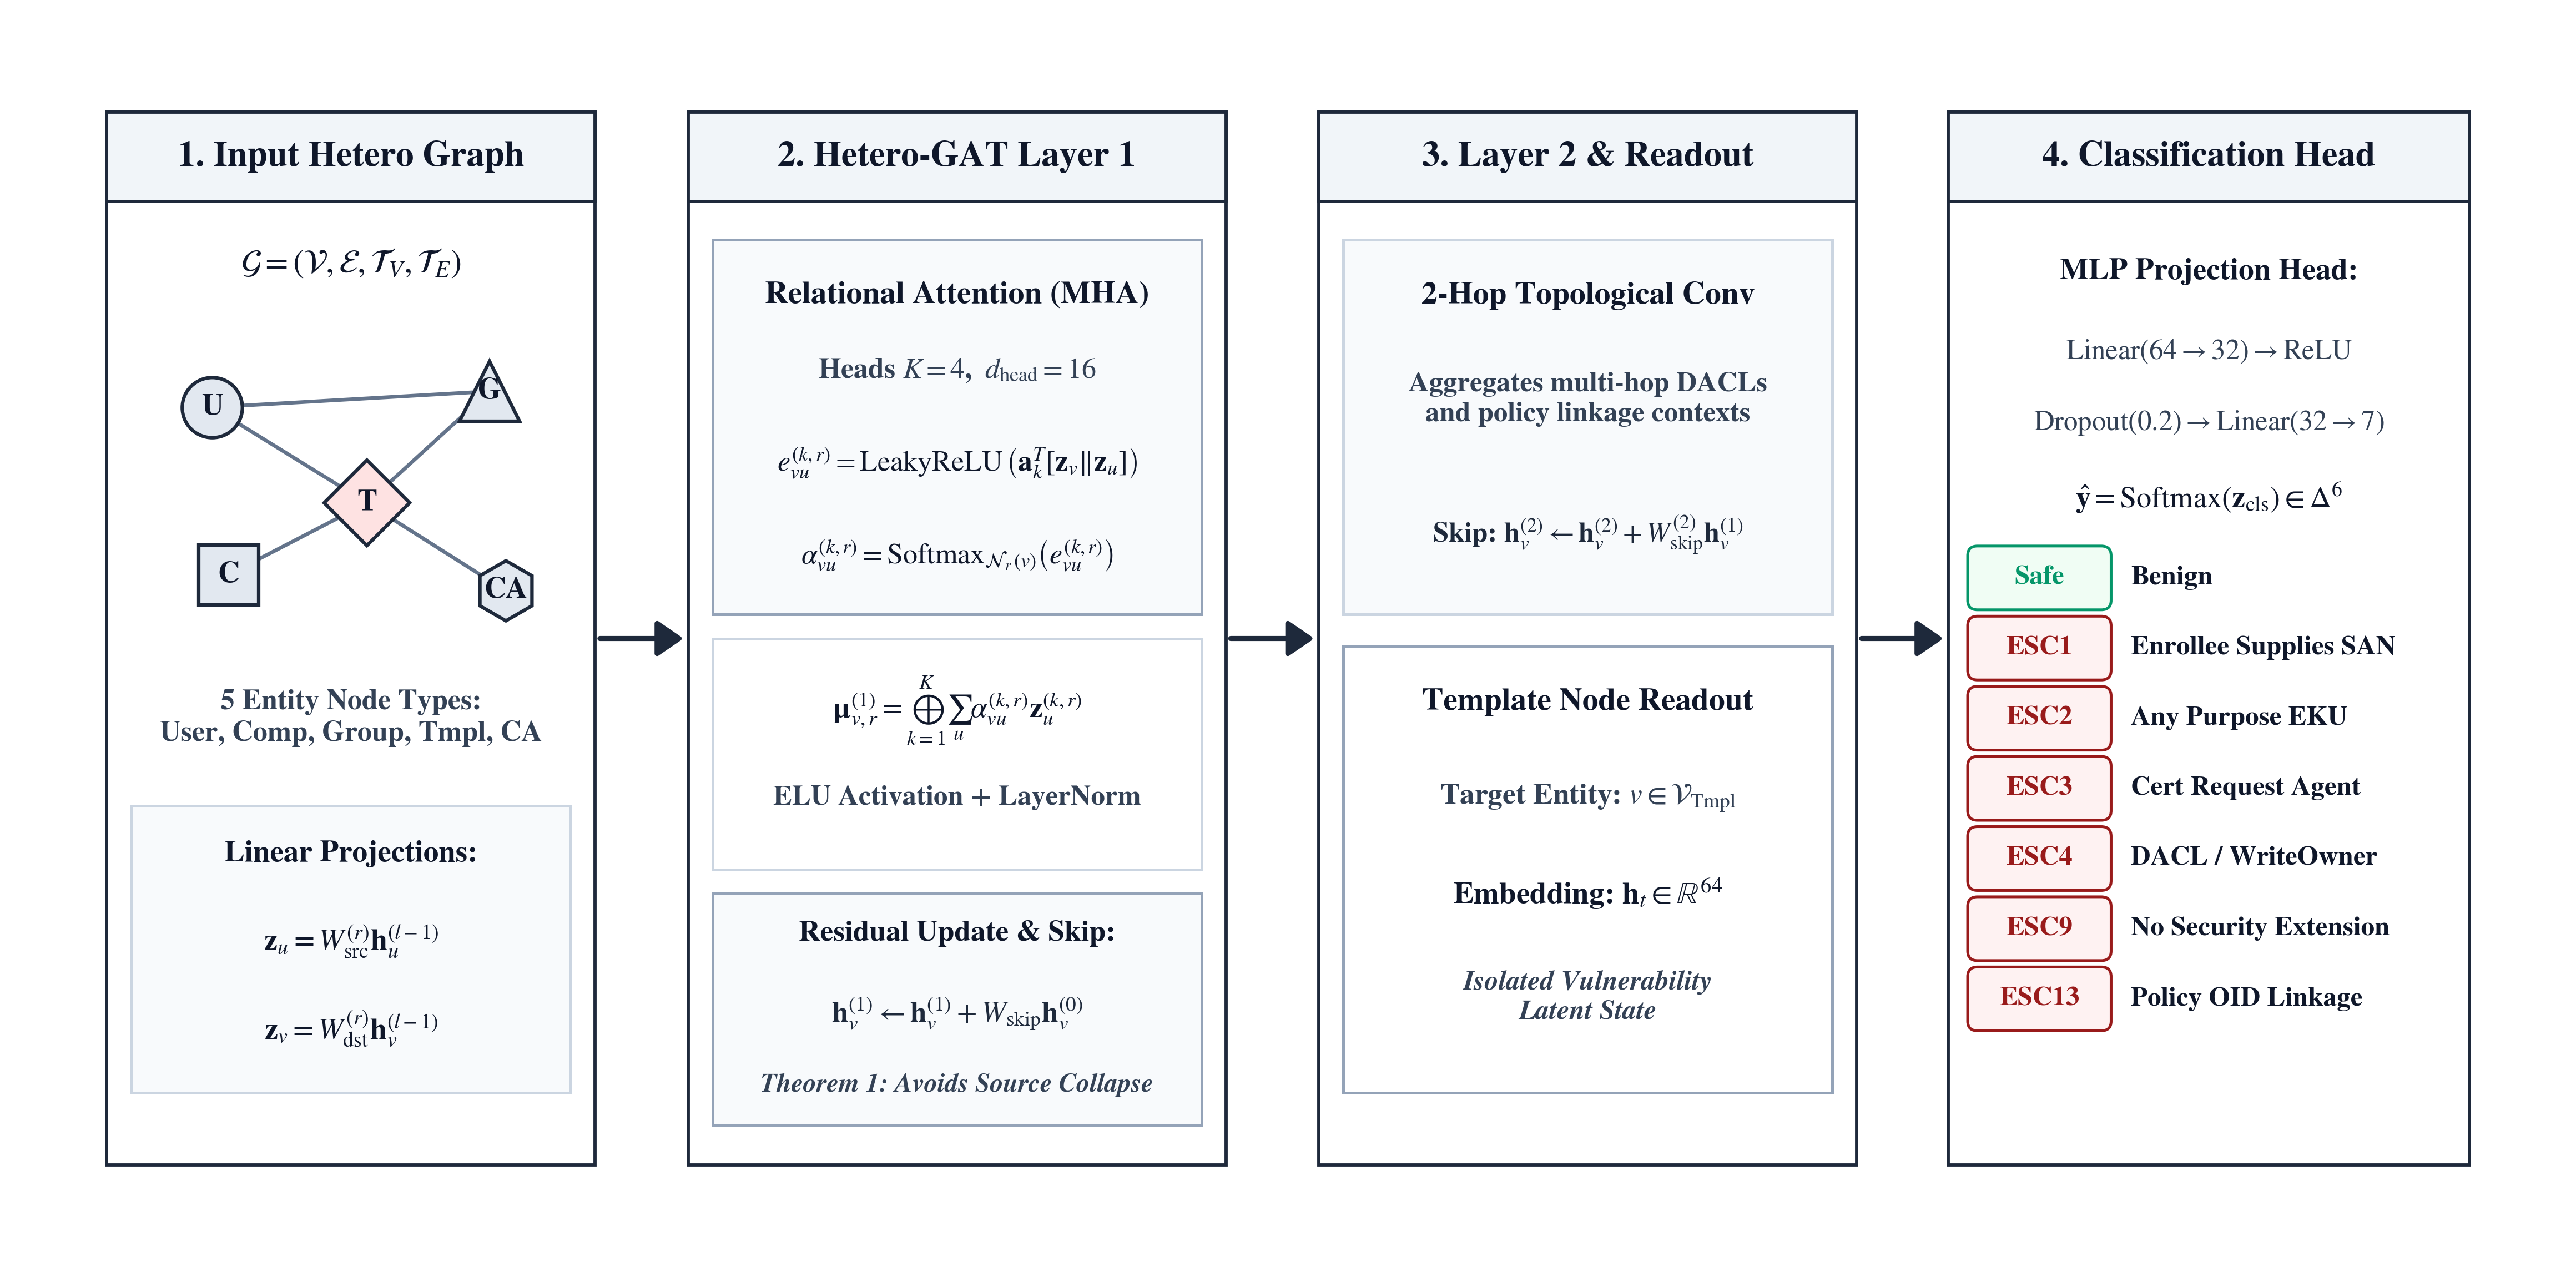
\includegraphics[width=0.98\textwidth]{figures/certgraph_architecture_diagram.png}
    \caption{CertGraph end-to-end Hetero-GAT pipeline, detailing input feature encoding, multi-head relational attention layers, additive residual skip-connections, and the multi-class template classification head.}
    \label{fig:certgraph_arch}
\end{figure}

\subsection{Relation-Specific Multi-Head Graph Attention}
Let $h_u^{(l-1)} \in \mathbb{R}^{d_{\tau(u)}^{(l-1)}}$ denote the hidden representation of node $u$ at layer $l-1$. For a directed relation $r = (\tau(u), \text{rel}, \tau(v))$ terminating at target node $v$, we project source and target features via relation-specific linear transformation matrices:
\begin{equation}
z_u^{(l, r)} = W_{\text{src}}^{(l, r)} h_u^{(l-1)}, \quad z_v^{(l, r)} = W_{\text{dst}}^{(l, r)} h_v^{(l-1)}
\end{equation}
where $W_{\text{src}}^{(l, r)} \in \mathbb{R}^{d_{\text{out}}^{(l)} \times d_{\tau(u)}^{(l-1)}}$ and $W_{\text{dst}}^{(l, r)} \in \mathbb{R}^{d_{\text{out}}^{(l)} \times d_{\tau(v)}^{(l-1)}}$.

To capture multi-faceted structural dependencies, we deploy $K$ independent attention heads. For head $k \in \{1, \dots, K\}$, the unnormalized attention coefficient $e_{vu}^{(k, r)}$ quantifying the importance of node $u$ to node $v$ across relation $r$ is:
\begin{equation}
e_{vu}^{(k, r)} = \operatorname{LeakyReLU} \left( \mathbf{a}_k^{(l, r) T} \left[ z_v^{(k, l, r)} \,\|\, z_u^{(k, l, r)} \right] \right)
\end{equation}
where $\mathbf{a}_k^{(l, r)} \in \mathbb{R}^{2 d_{\text{head}}}$ is the parameterized attention vector, and $\|$ denotes vector concatenation.

Normalized attention weights $\alpha_{vu}^{(k, r)}$ are computed via relation-level softmax over all incoming neighbors $\mathcal{N}_r(v)$:
\begin{equation}
\alpha_{vu}^{(k, r)} = \frac{\exp \left( e_{vu}^{(k, r)} \right)}{\sum_{w \in \mathcal{N}_r(v)} \exp \left( e_{vw}^{(k, r)} \right)}
\end{equation}

The aggregated representation of node $v$ under relation $r$ is the multi-head concatenation:
\begin{equation}
\mu_{v, r}^{(l)} = \prod_{k=1}^K \left( \sum_{u \in \mathcal{N}_r(v)} \alpha_{vu}^{(k, r)} z_u^{(k, l, r)} \right)
\end{equation}

\subsection{Semantic-Level Aggregation and Residual Skip-Connections}
Because target node $v$ may receive messages from multiple distinct incoming relation types $\mathcal{R}_{\text{in}}(\tau(v))$, CertGraph computes semantic-level aggregation via vector summation:
\begin{equation}
h_{v, \text{agg}}^{(l)} = \sum_{r \in \mathcal{R}_{\text{in}}(\tau(v))} \mu_{v, r}^{(l)}
\end{equation}

\paragraph{Crucial Residual Skip Connection:}
To prevent representation collapse and preserve node-specific attributes across message-passing iterations, we introduce parameterized additive residual skip-connections:
\begin{equation}
h_v^{(l)} = \operatorname{ELU} \left( h_{v, \text{agg}}^{(l)} + W_{\text{skip}}^{(l, \tau(v))} h_v^{(l-1)} \right)
\end{equation}
where $W_{\text{skip}}^{(l, \tau(v))} \in \mathbb{R}^{d_{\text{out}}^{(l)} \times d_{\tau(v)}^{(l-1)}}$ is a type-specific linear projection. Each convolution layer is followed by Layer Normalization and Dropout ($p = 0.2$).

\subsection{Multi-Class Vulnerability Classification Head}
After $L = 2$ message passing layers (providing a 2-hop receptive field sufficient to capture indirect delegation and issuance policy chains), we isolate the target certificate template embedding $h_{\text{target}}^{(L)} \in \mathbb{R}^{64}$. 

The embedding is passed through a Multi-Layer Perceptron (MLP) classification head:
\begin{align}
\tilde{z} &= \operatorname{ReLU} \left( W_1 h_{\text{target}}^{(L)} + b_1 \right), \quad W_1 \in \mathbb{R}^{32 \times 64} \\
\hat{y} &= \operatorname{Softmax} \left( W_2 \tilde{z} + b_2 \right), \quad W_2 \in \mathbb{R}^{7 \times 32}
\end{align}
where $\hat{y} \in \Delta^6$ is the predicted probability distribution over the 7 target classes:
\begin{equation}
\mathcal{C} = \{\text{Safe}, \text{ESC1}, \text{ESC2}, \text{ESC3}, \text{ESC4}, \text{ESC9}, \text{ESC13}\}
\end{equation}

The network is trained end-to-end by minimizing the Cross-Entropy loss with $L_2$ weight regularization:
\begin{equation}
\mathcal{L} = - \sum_{c=1}^7 y_c \log \hat{y}_c + \lambda \sum_{\theta \in \Theta} \|\theta\|_2^2
\end{equation}

\section{Theoretical Analysis: Representation Collapse in Directed Graphs}
A foundational theoretical contribution of this research is the formal mathematical proof that residual skip-connections are not merely an optimization heuristic in enterprise identity graphs, but a strict mathematical requirement.

\begin{theorem}[Representation Collapse of Source-Only Entities]
In any directed heterogeneous graph $G = (V, E, \mathcal{T}_V, \mathcal{T}_E)$ where a subset of node types $\mathcal{T}_{\text{source}}$ possesses zero incoming edges ($d_{\text{in}}(v) = 0$ for all $v \in V$ with $\tau(v) \in \mathcal{T}_{\text{source}}$), an $L$-layer heterogeneous message-passing neural network lacking residual skip-connections collapses the representations of all source-only nodes to the zero vector:
\begin{equation}
h_v^{(l)} = \mathbf{0}, \quad \forall v \in \mathcal{T}_{\text{source}}, \forall l \ge 1
\end{equation}
Furthermore, the gradient of the loss $\mathcal{L}$ with respect to the input features $x_v$ vanishes identically ($\frac{\partial \mathcal{L}}{\partial x_v} = \mathbf{0}$).
\end{theorem}

\noindent\textit{Proof.} The full formal proof is provided in Section~\ref{proof:theorem1}.

\begin{corollary}
In Active Directory graphs, user and workstation accounts frequently exhibit pure source topology in administrative authorization subgraphs. Omitting skip connections mathematically guarantees that the network becomes entirely blind to whether an enroller account is a privileged administrator or an unprivileged guest, destroying model capacity.
\end{corollary}
